%======================================================================
\chapter{Fast Motif Recognition via Statistical Thresholds} \label{chapter:pmclwmr}
%======================================================================


MCL-WMR uses graph clustering to determine pairwise bounded sets that might be valid motifs.  The major impediment to the efficiency of MCL-WMR was the exponential-time refinement algorithm used to determine which ``candidate motif sets'' ({\em i.e.}\ pairwise bounded sets) have a center string; this step becomes a bottleneck for solving challenging weak motif instances, such as $(18,6)$, when the number of such candidate sets increases dramatically \cite{BT02}.  In Chapter \ref{chapter:closest_string_problem}, we give a probabilistic heuristic for solving the {\sc Closest String} problem, which filters candidate sets based on a majority vote string, that has acceptable accuracy when $n$ is significantly large ({\em i.e.}\ when $n \geq 20$).  In this chapter, we propose a probabilistic algorithm that eliminates the need for a strong bound on $n$; our algorithm uses the weight of the set to determine quickly and with a small probability of error whether the set is a decoy set or a motif set.

We defined the weight of a set of strings $S$ as the sum of the pairwise Hamming distances, {\em i.e.}\ $\sum_{1\leq i<j\leq n} H(s_i, s_j)$. If the weight of a set, which can be calculated in polynomial time, can be used to indicate whether it is a motif set or a decoy set then the {\sc Closest String} string can be solved extremely efficiently and accurately in practice -- simply calculate the weight of the pairwise bounded set and decide whether the set has a center string based on this value.  For this heuristic to work we need to know how the respective weights of a random motif set and a random decoy set are distributed.  Further, the distributions need to be adequately separated so that the weight of a set leaves little ambiguity as to whether the set is a motif set or a decoy set.  

There exists an algorithm to sample from the set of all motif sets: simply choose any length-$\ell$ string as the center string and sample with replacement from the set of all strings that are at distance at most $d$ from that sequence. This sampling algorithm and its appropriateness was discussed in Chapter \ref{chapter:mclwmr}.  Unfortunately we do not know an analogous sampling algorithm, either exact or approximate, for decoy sets.  If we could sample pairwise bounded sets uniformly at random, then we could learn the probability distribution of the weight of a random decoy set.

We give a method to generate pairwise bounded sets uniformly, use this method to determine the probability distribution of the weight of a random decoy set, and show the existence of a separation between this distribution and the probability distribution of the weight of a random motif set.  Thus, we solve {\sc Closest String} instances accurately and efficiently using the simple heuristic of using the weight as an indicator as to whether a pairwise bounded set is a motif set or a decoy set.  The separation of the distributions becomes increasingly more prevalent as the number of strings in the set ({\em i.e.}\ the parameter $n$) increases, so the accuracy of our method increases as the number of strings increases.  

We significantly extend our earlier motif-recognition program, MCL-WMR, by incorporating the heuristic for the {\sc Closest String} problem described in this chapter. This new algorithm,  {\em sMCL-WMR}, detects motifs in data sets with a large number of strings ({\em i.e.}\ 30 or more strings).  sMCL-WMR represents the input data as a weighted graph and uses graph clustering to narrow the search to smaller problems that can be solved with significantly less computation.  An efficient refinement algorithm that distinguishes valid motif sets from decoy sets allows sMCL-WMR to detect motifs in very large data sets in significantly less computational time than MCL-WMR. 

Finally, we illustrate the applicability of sMCL-WMR and another variant, MCL-FSP, in analyzing the genomic data of canola.  Using these programs, we identify more than 40 motifs in promoters conjectured to be responsible for seed coat-specificity. Based on these motifs, a promoter DNA sequence of approximately 700 bp was synthesized and introduced into canola with the aim of obtaining its biological expression.

\section{Sampling Pairwise Bounded Sets} \label{sampling_sect}

We discuss uniform sampling, or generation, of pairwise bounded sets.  A standard method used to generate a random motif set is to choose an length-$\ell$ string uniformly at random from all possible $4^{\ell}$ strings to be the center string, and then form a motif set by selecting $n$ strings at random with replacement from the set of all strings with Hamming distance at most $d$ from this center string \cite{boucher07,BT02}.  This method samples a motif set uniformly at random, and further corresponds to how synthetic problem data sets are constructed.  For example, synthetic problem instances are traditionally generated as follows: a random center string of length $\ell$ is chosen, $n$ occurrences of the motif are generated by randomly mutating at most $d$ positions, and each of the $n$ motif instances is embedded at a random location into a different background string of length $m$.  We note that other non-uniform distributions have also been used to generate motif sets \cite{PS00}. 

When sampling uniformly from a poorly understood sample set, {\em rejection sampling} is a na\"{\i}ve but useful technique.  If we can find a superset of the target set that is easy to sample from uniformly, we can sample from this superset and simply throw away (reject) any sampled element that is not in the target set.  To sample uniformly at random from all pairwise bounded sets using rejection sampling in the most na\"{\i}ve way, we would generate $n$ random length-$\ell$ strings and accept the set if it is pairwise bounded, and reject and repeat otherwise.  However, since it is unlikely that such a randomly generated set would be pairwise bounded, this method is extremely inefficient.  We introduce a heuristic to generate random sets that are more likely to be pairwise bounded, thus speeding up the rejection sampling process enough to be practical.

We generate the first string, $s_1$, uniformly at random from the set of all length-$\ell$ strings then generate each of $s_2,\ldots,s_n$ in turn uniformly at random from the set of all strings at distance at most $2d$ from $s_1$.  This gives us a set of strings generated uniformly at random from the set of all strings that have $s_1$ as the first string and each other string at distance at most $2d$ from $s_1$.  If the set is pairwise bounded we keep it; if it is not we reject it and start over.  The fact that this method generates pairwise bounded sequences uniformly at random can be verified by induction on $n$.

The number of times a set of $n$ strings is considered and rejected until a pairwise bounded set is generated follows a geometric distribution and therefore, the efficiency of this method is determined by the probability that a set is rejected.  Though this method is fast enough to work in practice for values of $n$ we are interested in, the expected running time when generating a single pairwise bounded set grows exponentially with $n$.

\begin{definition} {\bf (Neighbourhood)} For a string $s \in \Sigma^{\ell}$, the $(\ell, k)$-neighbourhood of $s$, denoted as $N_{\ell, k}$, is the set $$\{ s_i | s_i \in \Sigma^{\ell}, d(s_i, s) \leq k \}.$$ \end{definition}

\noindent We note that $|N_{\ell, k}| = \sum_{i = 0}^{k} {{\ell}\choose{k}}(|\Sigma| - 1)^{k}$.  

\begin{proposition} The probability that a set generated using the above method is pairwise bounded decreases at least exponentially fast as a function of $n$. \end{proposition}
\begin{proof}
For $1\leq i\leq n$ let $S_i$ be the subset of $S$ containing the first $i$ randomly chosen strings, with $S_n=S$.  Let $A_i$ be the event that $S_i$ is pairwise bounded.  Any subset of a pairwise bounded set is pairwise bounded, so $A_i$ implies $A_{i-1}$ for $2\leq i\leq n$.  Therefore by Bayes' law we have $\Pr(A_i)=\Pr(A_i|A_{i-1})\Pr(A_{i-1})$.  To prove that $\Pr(A_n)$ decays exponentially with $n$ we need only show that $\Pr(A_i | A_{i-1})$ is non-increasing in $i$, since it can easily be verified to be strictly less than 1 for $i=3$.  Let $K_i$ be the set of strings such that $S_i\cup\{s\}$ is pairwise bounded if and only if $s\in K_i$, noting that $K_i = \emptyset$ if $S_i$ is not pairwise bounded.  We have $K_j\subseteq K_i$ for any $1\leq i<j\leq n$.  Since $\Pr(A_i | A_{i-1}) = \frac{|K_i|}{N_{\ell, 2d}}$, the result holds. \hfill $\Box$ \end{proof}

Further, the probability that the set is not rejected is equal to $\left( \frac{N_{\ell, 2d}}{|\Sigma|^{\ell}}\right)^{n - 1}$.  To empirically evaluate the efficiency of our rejection sampling method, we determined the portion of sets that will be rejected when generating a sample (of specified size) of pairwise bounded sets.  We performed experiments with varying values of $n$, $\ell$, and $d$, generated $10000$ pairwise bounded sets in each experiment, and considered the average number of sets rejected before the pairwise bounded set was obtained.  The default values for $(n,\ell,d)$ are $(20,15,4)$. 


\begin{figure}[h]
\begin{center} 
 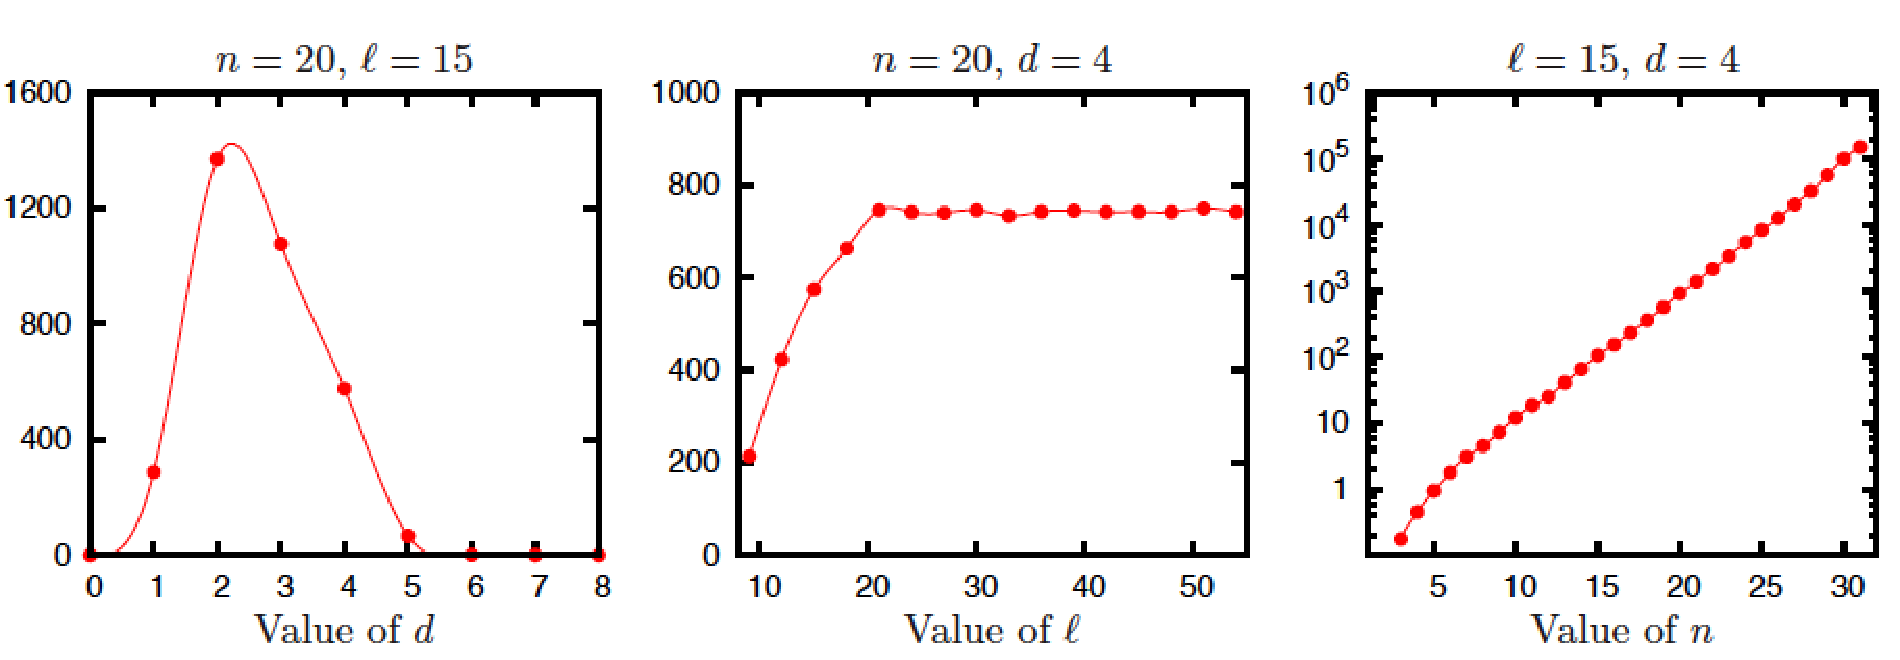
\includegraphics[width=\linewidth]{images/temp}
\caption[Data illustrating the mean number of sets rejected by our rejection sampling heuristic in order to generate a pairwise bounded set.]{Data illustrating the mean number of sets rejected by our rejection sampling heuristic in order to generate a pairwise bounded set. Each plot shows the affect of varying one of the three parameters $n$, $\ell$, and $d$.  Data points are connected with cubic splines.  Note the logarithmic scale used in the right plot.}
\label{fig:separation}
\end{center}
\end{figure}

 The results of the empirical tests are shown in Figure \ref{fig:separation}.  Each of the three plots shows how the average number of rejected sets changes when one of the three parameters is varied and the other two are fixed at their default values.  The left plot shows what happens when $d$ varies between $1$ to $7$.  For values of $d$ that are either greater than $\lfloor \ell /2 \rfloor$ or equal to $0$, any set we generate is pairwise bounded and hence, we did not plot data for $d = 0$ or $d \geq 8$.  The average number of rejected sets is largest when $d$ is equal to 2 and decreases dramatically as $d$ increases. This trend is expected since a large portion of non-pairwise bounded sets would be rejected when $d$ is moderately large.  The middle plot shows what happens when $\ell$ is varied between 9 and 55.  The number of rejected sets increases steadily when $\ell$ varies within the range $[9, 20]$, then plateaus when $\ell$ is above 20.  It can be easily shown analytically that increasing $\ell$ above $2dn$ will have no effect, however, we see empirically that the effect of $\ell$ is minimal for values of $\ell$ greater than 20.  The right plot shows the effect of varying $n$ between $3$ and $31$.  Noting that a logarithmic scale is used, the average number of rejected sets exhibits growth that is clearly exponential in $n$.



%%%%%%%%%%%%%%%%%%%%%%%%%%%%%%%%%%%%%%%%%%%%%%%%%%%%%%%%%%%%%%%%%

\subsection{A Separation of Weight Distributions}

One of the key motivations for the development of methods to generate pairwise bounded sets from an appropriate distribution is that it can be used to determine whether there is a separation between the probability distribution of the weight of a random valid motif set and that of a random decoy set. We use the sampling method just described to generate 1000 random motif sets and 1000 random decoy sets for varying values of $\ell$, $d$, and $n$.  We ran the sampling algorithm described above to generate a pairwise bounded set then determined whether it is a motif set or a decoy set by using the dynamic programming algorithm described in Chapter \ref{chapter:mclwmr}.  We continued generating pairwise bounded sets until we obtained 1000 decoy sets and 1000 motif sets.  For each random motif and decoy set witnessed we calculated the weight of the set.  Figure \ref{fig:separation2} depicts, for values considered for $\ell$, $d$, and $n$, the distribution of the weight of the 1000 random motif sets and that of the 1000 random decoy sets.  The data illustrate an adequate separation between the distributions.  

As the value of $n$ increases, the separation between the distributions becomes more prevalent since the probability distributions become more concentrated around their means and the means themselves diverge.  Further, the dichotomy is again more evident when $(\ell, d)$ is increased from $(15, 4)$ to $(18, 6)$. When $n$ is even moderately large we can use the weight to determine accurately whether the set is a motif set or a decoy set and as $n$ increases this method of using the weight as an indicator will likely increase in accuracy.  Similar conclusions can be made when $\ell$ and $d$ increase. These results suggest that the simple heuristic of using the weight to determine whether a pairwise bounded set is a valid motif set or a decoy set will enable computationally challenging instances of the {\sc Closest String} problem ({\em e.g.}\ when $n \geq 20$ or $(\ell, d)$ is equal to $(18, 6)$) to be solved efficiently with minimal probability of error.


\begin{figure}[h!]
\begin{center} 
 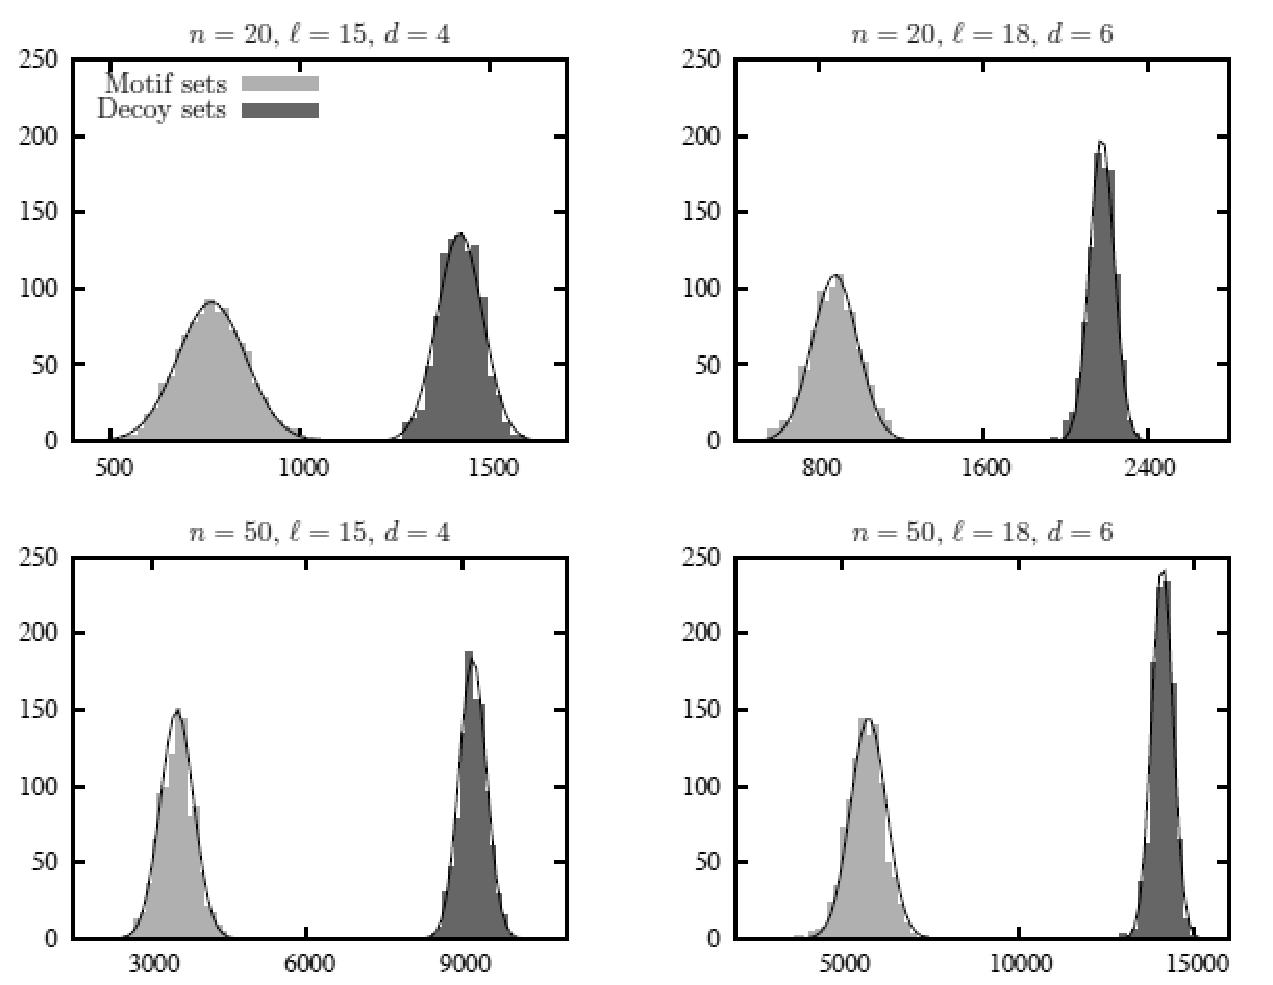
\includegraphics[width=\linewidth]{images/temp2_b_w}
 \caption[Data showing the distribution of the weight of a random motif set, and that of a random decoy set.]{Data showing the distribution of the weight of a random motif set, and that of a random decoy set. Normal distributions fitted to the data are shown to indicate that the weight distributions are approximately normal.}
\label{fig:separation2}
\end{center}
\end{figure}

These empirical trends illustrate the analytical results proved in Chapter \ref{chapter:mclwmr} that demonstrate that the distribution of the weight of a random motif set is tightly concentrated around its mean. It is currently an open problem to prove an analogous result to Theorem \ref{azuma_thm} in Section \ref{section:mcl_wmr_analysis} for an arbitrary decoy set.  This is a considerably more challenging problem due to the lack of a combinatorial characterization of a decoy set.  

%%%%%%%%%%%%%%%%%%%%%%%%%%%%%%%%%%%%%%%%%%%%%%%%%%%%%%%%%%%%%%%%%
\section{An Overview of sMCL-WMR} \label{smcl_wmr_tail_values}

sMCL-WMR considers a weighted graph representation of the input data (as MCL-WMR does), and then uses MCL) \cite{vD00} to cluster the resulting graph. The construction of our graph $\mathcal{G}$ ensures that the motif instances represented by vertices in the graph are connected to each other and form a clique of size $n$, though the converse need not hold. Thus, the problem of finding pairwise bounded sets in the data reduces to finding cliques of size $n$ in the graph $\mathcal{G}$.  Next, we filter out the clusters produced by MCL that do not meet the criteria of having at least $n$ vertices or the minimum weight threshold. See Section \ref{section:mcl_wmr_system} for the details of the construction of the graph and the graph clustering algorithm.  

Figure \ref{fig:separation2} illustrates that both the weight of a random motif set and that of a random decoy set are approximately normally distributed, and shows a separation between these distributions.  Using the rejection sampling method described earlier we calculate the mean and standard deviation of the weight of a random motif set and the weight of a random decoy set. We use $N(\mu, \sigma^2)$ to denote a normal distribution with mean $\mu$ and variance $\sigma^2$.  Let random variables $W_m$ and $W_d$ denote the weight of a random motif set and the weight of a random decoy set, respectively. Let $\mu_m$ and $\sigma_m^2$ respectively denote the mean and variance of the distribution of $W_m$ and similarly, let $\mu_d$ and $\sigma^2_d$ respectively denote the mean and variance of $W_d$.  Assuming that $W_m \sim N(\mu_m, \sigma_m^2)$ and $W_d \sim N(\mu_d, \sigma_d^2)$, we can determine the values $\alpha_m$ and $\alpha_d$ such that: $$\Pr(W_m < \alpha_m) = .99 \mbox{ and } \Pr(W_d > \alpha_d) = .99~.$$ If $\alpha_m < \alpha_d$ then we can use the weight of a pairwise bounded set of strings to determine whether the set is a decoy or a motif as follows: calculate the weight $w$ of the set and, if $w \leq \alpha_m$ or  $w \geq \alpha_d$ then return that the set is a motif or a decoy, respectively; otherwise, use the dynamic-programming algorithm to classify the set.  Hence, if $\alpha_m < \alpha_d$ then more than 99\% of pairwise bounded sets will be classified correctly by considering the weight of the set.  Typically the gap between $\alpha_m$ and $\alpha_d$ is large enough to guarantee that this rate is far higher than 99\%.  In theory it is possible that a set could be misclassified ({\it e.g.}\ if a motif set has weight greater than $\alpha_d$) though in practice the probability of this happening is negligible and does not affect the performance of the algorithm.



\begin{table}[h!]
  \begin{center}
	\begin{tabular}{|c|c|c|c|c|c|c|}
\hline	
$(\ell, d)$& $\mu_m$ & $\mu_d$ & $\sigma_m^2$ & $\sigma_d^2$ & $\alpha_m$ & $\alpha_d$ \\
\hline
\hline
(15, 4)	& 794  		& 1439 	& 84    		& 84    		& 989 		& 1243		 \\
(16, 5) 	& 850 		& 1651 	& 86    		& 102  		& 1050 	& 1413		\\
(18, 6) 	& 899 		& 2204 	& 89    		& 140		& 1106 	& 1878 	 \\
(25, 8)	& 954 		& 2670 	& 111   	& 175  		& 1212 	& 2262		\\
(28, 9)	& 1024 	& 3230 	& 152   	& 199 		& 1378		& 2767		\\
(30, 11)& 1069 	& 3882 	& 169   	& 245 		& 1462		& 3312		 \\
	\hline
	\end{tabular} 
\caption[Data illustrating the mean and standard deviation of the weight of a random motif set and the weight of a random decoy set for various $(\ell, d)$-motif problems.]{Data illustrating the mean and standard deviation of the weight of a random motif set and the weight of a random decoy set for various $(\ell, d)$-motif problems.  The number of strings is fixed at 20.}
\label{chapter6:table3}
\end{center}
\end{table}


\begin{table}[h!]
  \begin{center}
	\begin{tabular}{|c|c|c|c|c|c|c|}
\hline	
$n$ & $\mu_m$ & $\mu_d$ & $\sigma_m^2$ & $\sigma_d^2$ & $\alpha_m$ & $\alpha_d$ \\
\hline
\hline
15 	& 432  	& 980 		& 52  		& 60    	& 552   	& 840  \\
20 	& 794  	& 1439 	& 84  		& 84    	& 989  		& 1243	\\
25 	& 1529 & 2250 	& 129 		& 110	& 1829		& 1994 \\
30 	& 1845 & 3263 	& 196 		& 169  	& 2300 	& 2869\\
35 	& 2240 & 4523 	& 246 		& 213   & 2812 	& 4027 \\
40 	& 3709 & 6110 	& 389 		& 275   & 4613  	& 5460 \\
	\hline
	\end{tabular} 
\caption[Data illustrating the mean and standard deviation of the weight of a random motif set and the weight of a random decoy set for various values of $n$.]{Data illustrating the mean and standard deviation of the weight of a random motif set and the weight of a random decoy set  for various values of $n$. The values $\ell$ and $d$ are fixed at $15$ and $4$, respectively.}
\label{chapter6:table4}
\end{center}
\end{table}

To increase the efficiency of sMCL-WMR, we include a pre-calculated table storing $\mu_m$, $\mu_d$, $\sigma_m^2$ and $\sigma_d^2$ for common values of $\ell$, $d$, and $n$ (for examples see Table \ref{chapter6:table3} and \ref{chapter6:table4}).  We varied $n$ to be between 10 and 50, $\ell$ to be between $15$ and $30$, and $d$ to be between $\lfloor \ell/5\rfloor$ and $\lfloor \ell/2\rfloor$.  Values with weaker motifs or with small data sets ({\em i.e.}\ when $n \leq 10$) are not considered since it was shown that MCL-WMR performs efficiently for these instances. 


%%%%%%%%%%%%%%%%%%%%%%%%%%%%%%%%%%%%%%%%%%%%%%%%%%%%%%%%%%%%%%%%%
\section{An Overview of MCL-FSP}

In many practical applications -- including the analysis of the genetic data in this chapter -- we are not only interested in identifying strings whose maximum distance from each the given strings is minimized but also in identifying strings whose minimum distance from each of the given strings is maximized.  Given a set $S_f$ of strings of length at least $\ell$ over an alphabet $\Sigma$ and a non-negative parameter $d_f$,  the objective of the {\sc Farthest String} problem is to determine if there exists a string $s$ over the alphabet $\Sigma$  such that for any $s_i \in S_f$, $d(s, s_i) \geq d_f$.   We refer to the subsequences occurring in the input sequences as {\em non-motifs}.

We describe a program, {\em MCL-FSP}, that given $n$ length-$m$ sequences over the alphabet $\Sigma$ and parameters $\ell$ and $d$, finds substrings of length $\ell$ in the input data and a length-$\ell$ string $s$ where the goal of the {\sc Farthest String} problem is satisfied with respect to the parameters $\ell$ and $d$.  MCL-FSP can be summarized by the following three steps: graph construction, graph clustering, and recovering the instances and their farthest string.  The graph construction and clustering is similar to MCL-WMR and sMCL-WMR. However, the recovering of the substrings of interest is dramatically different.  The graph constructed for MCL-FSP builds the same set of vertices but joins each pair of vertices by an edge if the Hamming distance between the strings corresponding to the pair of vertices is less than or equal to $d$.  The weight on each edge is $\ell$ minus the Hamming distance between the corresponding strings of the endpoints of the edge.  There exists no additional weighting on the edges. 

The clustering of the graph will yield dense clusters in the graph.  These dense subgraphs will likely contain a set of $n$ substrings that are ``close'' -- meaning the pairwise Hamming distances are small -- and hence, are likely to have a string $s$, which satisfies the {\sc Farthest String} problem together with the set of $n$ substrings.

To recover sets on substrings that satisfy the {\sc Farthest String} problem we first filter out clusters that do not have a substring from each of the input and clusters whose weight is less than $d \cdot {n \choose 2}$. Clusters that pass this test may contain multiple cliques formed by choosing different subsets of $n$ cluster vertices, or possibly no cliques at all. We identify all ways of forming a clique from the cluster vertices by using the $n$-partite nature of the graph to explore all possible cliques with a depth-first search. For each such clique, we use Algorithm \ref{alg:FSP} to determine whether the substrings in the clique correspond to a valid {\sc Farthest String} solution.

\begin{algorithm}[h]
\caption{FSP Recovery Algorithm}
\begin{algorithmic}
\STATE {\bf Input: } A set of $S$ $n$ strings of length $\ell$, parameters $\Delta d$ and $d$, and a candidate string $x$.
\STATE {\bf Output:} A string $s^*$ with the minimum distance to any string in $S$ at least $d$ if it exists and ``Not found'' otherwise.
\STATE If $\Delta d < 0$ then return ``Not found''
\STATE Choose $i \in \{1, \ldots, n\}$ such that $d(x, s_i) < d$. If no such $i$ exists return $x$.
\STATE \hspace{5mm} $\mathcal{P} = \{p \, |  \, x[p] = s_i[p]\}$;
\STATE \hspace{5mm} Choose any $\mathcal{P}'$ from $\mathcal{P}$ with $|\mathcal{P}'| = \ell - d + 1$.
\STATE \hspace{5mm} For each position $p \in \mathcal{P}'$
\STATE \hspace{10mm} Let $x$ not be equal to $s_i$ at position $p$ 
\STATE \hspace{10mm} $s_{ret}$ = FSP Recovery Algorithm ($S$, $\Delta d - 1$, $x$) 
\STATE \hspace{10mm} If $s_{ret} \neq $ ``not found '', then return $s_{ret}$
\STATE Return ``not found''
\end{algorithmic}
\label{alg:FSP}
\end{algorithm}

As mentioned previously, the {\sc Farthest String} problem is NP-complete and therefore, unlikely to be solved in polynomial time. Algorithm \ref{alg:FSP} is based on the bounded search tree algorithm of Gramm {\em et al.}\ \cite{GNR03} for the {\sc Closest String} problem, and has been previously studied by Cheng {\em et al.}\ \cite{cheng}.  Cheng {\em et al.}\ \cite{cheng} proved Algorithm \ref{alg:FSP} has a worst-case running time of $O((|\Sigma|(\ell - d)^{\ell - d})$ and is guaranteed to solve {\sc Farthest String} instances exactly.  

%%%%%%%%%%%%%%%%%%%%%%%%%%%%%%%%%%%%%%%%%%%%%%%%%%%%%%%%%%%%%%%%%

\section{Experimental Results on Synthetic Data}

We tested sMCL-WMR and MCL-FSP on synthetic problem instances generated according to the embedded $(\ell, d)$-motif model, and on real genetic data. The implementations of sMCL-WMR and MCL-FSP are coded in C++, and all experimental tests were performed on a Linux machine with a 64-bit 2600 MHz processor and 1 Gbyte of RAM running Ubuntu.   The running time is given in CPU seconds.  

We follow the experimental methods of Pevzner and Sze \cite{PS00}, and Buhler and Tompa \cite{BT02} by considering the performance of sMCL-WMR and MCL-FSP in comparison to other contemporary and well-known motif-recognition programs on synthetic data.  We fix $n$ to be equal to 20, $m$ to be 600, and consider varied values of $\ell$ and $d$. To produce random motif-recognition instances, we generate a random center string of length $\ell$, then generate $n$ occurrences of the motif, each generated from the center string by randomly choosing $d$ positions and for each of the $d$ positions choosing a random replacement base from the four possible bases (A, C, G, T). We construct $n$ background strings of length $m$ and insert the generated motifs into a random position in the string.  For each of the $(\ell, d)$ combinations, 100 randomly generated sets of input strings were generated. 

We compared the performance of sMCL-WMR and MCL-FSP with that of the following motif-recognition programs: PROJECTION \cite{BT02}, MCL-WMR, PMSprune \cite{JBR07}, and Voting \cite{CL05}.  All programs were run on the same Linux machine with the same data sets.  These motif-recognition programs were chosen for their availability, performance, and widespread use; they are appropriate for comparison with sMCL-WMR because of the previously described capability in solving weak motif instances and because of their availability to be run on the described machine. The results of Voting, PMSprune, and PROJECTION are similar to the ones reported by Davila {\em et al.}\ \cite{JBR07}, and to Chin and Leung \cite{CL06}, both of whose testing was completed on a machine with a slightly slower processor and the same core memory size.  


\begin{table}[h!]
\begin{center} {
	\begin{tabular}{|c|c|c|c|c|c|c|c|}     
    \hline	
	$(\ell, d)$				& sMCL-WMR	 	& MCL-FSP	 	& MCL-WMR		& PROJECTION		& Voting		& PMSprune			\\
	\hline
    (10, 2)					& 122 					& 1131				& 1020 			& 560 (0.98)		& 30				& 42 					\\
	(12, 3)  				& 134 					& 3019				& 2780				& 1921 (0.85) 		& 124			& 130 					\\
	(14, 4)		 			& 492 					& 3325				& 3120				& 3058 (0.88)		& 562			& 556			 		\\
	(16, 5)					& 677 					& 4502				& 4101				& 6132 (0.80)		& 2600		  	& 13121					\\
	(18, 6)					& 1521 				& 8950				& 9202				& -						& 8023			& 29012  				\\
	(20, 7)					& 2845					& -					& -					& -						& 24600		& - 						\\
	(25, 8)				    & 4111 				& -					&	-					& -						&	-			 	& - 						\\
%	(28, 10)				& 2791 				& -					&	-					& -						&	-			   	& - 						\\
	\hline
	\end{tabular}}
\end{center}
\caption[Comparison of the performance of sMCL-WMR, MCL-FSP, and other motif-recognition programs on synthetic data for various values of $\ell$ and $d$.]{Comparison of the performance of sMCL-WMR, MCL-FSP, and other motif-recognition programs on synthetic data for various values of $\ell$ and $d$. All programs except PROJECTION had a success rate of 1.0 and for this reason, the success rate was for PROJECTION is included in brackets in the table. In all experiments, $m = 1000$ and $n = 20$.}
\label{smcl_wmr:compare1}
\end{table}


\begin{table}[h!]
\begin{center} {
	\begin{tabular}{|c|c|c|c|c|c|c|}     
	\hline	
	$n$			& sMCL-WMR	& MCL-FSP		& MCL-WMR		& PROJECTION		& Voting				& PMSprune\\
	\hline
    18			& 547 				& 5559				& 5320				&	5230 (0.85)		& 3930					& 37020 \\
	20  			& 679				& 8823				& 8912				&  -						& 5201					& 45030  \\
	24		  	& 1221 			& -					& -					&	-						& 10211				& - \\
	28			& 2019				& -					& -					&	-						&	-						& - \\
	30			& 2431		 		& -					& -					&	-						&	-						& - \\
	40			& 5201		 		& -					& -					&	-						&	-						& - \\
	\hline
	\end{tabular}}
	\end{center}
	\caption[Comparison of the performance of sMCL-WMR, MCL-FSP, and other motif-recognition programs on synthetic data for various values of $n$.]{Comparison of the performance of sMCL-WMR, MCL-FSP, and other motif-recognition programs on synthetic data for various values of $n$. All programs except PROJECTION had a success rate of 1.0 and for this reason, the success rate was for PROJECTION is included in brackets in the table.In all experiments, $\ell = 18$, $d = 6$ and $m = 1000$.}
\label{smcl_wmr:compare2}
\end{table}
	

Tables \ref{smcl_wmr:compare1} and \ref{smcl_wmr:compare2} illustrate the comparison between the running time of sMCL-WMR and that of the other programs.  Our aim was to test the selected programs on their capability to solve challenging motif instances ({\em i.e.}\ when $d$ is significantly large with respect to $\ell$).  The symbol ``-'' implies that the program was not capable of solving the motif instance on the described machine in a reasonable amount of time, which we define to be at most 20 hours, or with reasonable accuracy, which we define to be at least 75\%.  Two significant trends are witnessed in the data: sMCL-WMR is capable of solving very hard instances of motif recognition ({\em i.e.}\ when $\ell = 25$ and $d = 8$) and gives a dramatic improvement over the existing programs for instances where $\ell \geq 16$ (for instances where $\ell \leq 12$ sMCL-WMR had comparable or better performance to the other programs). MCL-FSP had a slightly higher running time than MCL-WMR and failed on the same instances as MCL-WMR. 


\section{Development of a Seed Coat-Specific Promoter for Canola}

Canola ({\em Brassica napus L.}) was originally bred from rapeseed in Canada in the 1970s \cite{downey}. Presently, the canola industry generates more than \$11 billion of yearly income to the Canadian economy. One of the major exports of the canola industry is {\em canola meal}, which is most widely used in animal feeds. However, one of the major problems with canola meal is the dark polyphenolic pigments that accumulate in the seed coat; the dark pigment interferes with the protein utilization, causing the quality of the meal to be lowered. Hence, altering the seed coat is an important biological challenge that has the possibility of reducing the indigestible fiber and enhancing the usability of canola meal.  One first step in  tackling this problem is to develop seed coat-specific promoters which are capable of regulating the genes involved in seed coat development and metabolism. 

One approach to finding seed coat-specific promoters for canola is to isolate the promoters of proved seed coat-specific genes from other species, and then validate their expression in canola.  Since genes are conserved among species, this is a reasonable approach.  Preliminary results identified that several promoters express in the outer integument of seed coat in canola, and a single promoter expresses in the inner integument. The subsequent challenge is to synthetically develop a promoter sequence that expresses both these two biological characteristics.  This synthetic promoter can then be artificially inserted into the genomes of the canola seeds and be tested for their expression. Table \ref{table:promoters} gives an overview of the relevant data concerning the promoter sequences analyzed.      
     
\begin{table}[h!]
\begin{center} {
\begin{tabular}{|l|c|cccc|}     
\hline	
Promoter		& bp		& \multicolumn{4}{c|}{Composition} \\		
					&						& A 			& C 			& G 			& T \\
\hline
\hline
 AtLAC15 		&1528 				& 33\%  	& 19\%  	& 16\% 	& 33\% \\
\hline
Arabidopsis BAN & 236 		& 33\%  	& 18\%  	 & 14\%  	& 34\% \\
\hline
VPE				& 2067 			& 34\%  	& 16\%  	& 17\%  	& 32\% \\
\hline
GILT 			& 2889 			& 36\%  	& 13\%  	& 14\%  	& 37\% \\
\hline
Arabidopsis TT12 & 1704	& 36\%  	&16\%  	& 17\%  	& 31\%\\
\hline
Arabidopsis TT2  & 3813 	& 38\%  	& 14\%   	& 14\%  	& 34\% \\
\hline
Barley Germin B gene & 846 & 35\% 	& 15\%		& 15\%		& 35\%\\
\hline
Tobacco Cryptic       & 2553 & 33\%  	& 18\%  	 & 14\%  	& 34\% \\
\hline
SCS1							& 7235 & 37\%  	& 12\% 	& 12\%  	& 39\% \\
\hline
SCB1 						& 5329	& 38\%		& 12\%		& 15\%		& 35\\ 
\hline
	\end{tabular}}
	\end{center}
	\caption[Description of promoters analyzed to develop a coat-specific promoter.]{Description of promoters analyzed to develop a coat-specific promoter.}
\label{table:promoters}
\end{table}


In order to use sMCL-WMR to find motifs in the genetic data we need to ensure that there exists a separation between the weight of the motif sets and decoy sets found in the data.  We have previously shown such a separation exists for synthetic data.  For a subset of the values of $n$, $\ell$ and $d$ that are to be used in the analysis, we ran MCL-WMR and calculated the weight of the motif sets and decoy sets found.  Figure \ref{fig:canola_separation} illustrates this data. For all values of $n$, $\ell$, and $d$ tested, there exists a clear separation between the distributions and we were able to use the precalculated tail values determined in Section \ref{smcl_wmr_tail_values}.

\begin{figure}[h!]
\centering
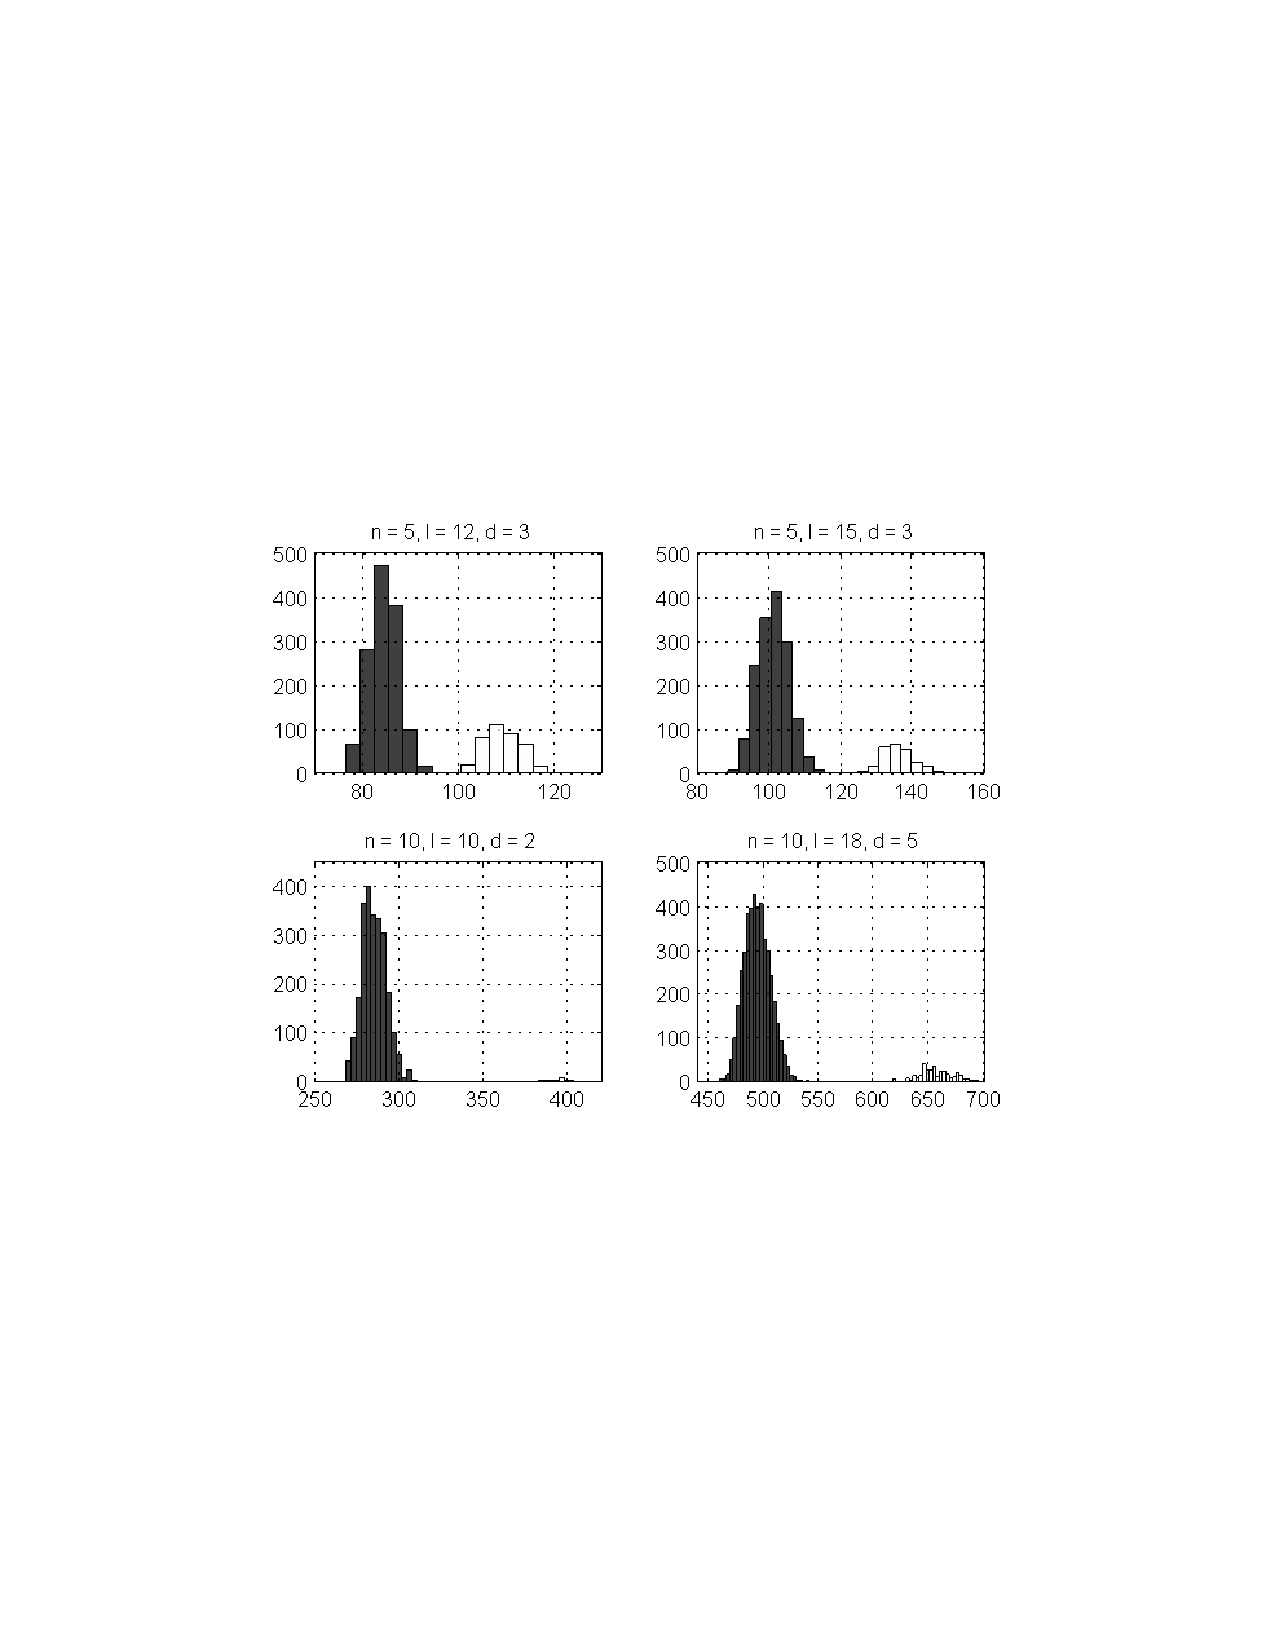
\includegraphics[width=90mm,trim=7cm 8cm 7cm 7cm]{images/canola_separation}% picture filename
 \caption[An Illustration of the distribution of the weight of a random motif set found in the promoter data, and that of a random decoy set found in the promoter data.]{An Illustration of the distribution of the weight of a random motif set found in the promoter data (shown in white), and that of a random decoy set found in the promoter data (shown in black). }
\label{fig:canola_separation}
\end{figure}


The conserved motifs were identified through the use of sMCL-WMR and MCL-FSP. Table \ref{table:detected_motifs} gives a subset of the motifs detected by sMCL-WMR and the CPU time in seconds for their detection.  In addition, it was of interest to identify furthest strings that were contained in one of the input sequences.  Table \ref{table:detected_nonmotifs} contains a sample of the furthest strings and which of the input sequences it occurs in; for the remaining sequences the specified string is a furthest string with respect to the parameters $\ell$ and $d$.  In particular, detecting furthest strings that occurred in one of the following three promoters was of interest: the AtLAC15, Arabidopsis BAN and Arabidopsis TT2 promoters.  

Each of these promoters has a specific biological role in the development of one of the different layers of seed coat. sMCL-WMR was used to determine the nucleotide patterns common to each of the promoters and hence, maybe responsible for having biological activity concerning the seed-coat. MCL-FSP was used to detect nucleotide patterns that were distinct to particular promoters that were responsible for the outer integument and inner integument of the seed coat -- in hope of identifying biological sequence patterns responsible for each specific seed-coat integument.  We identified more than 40 motifs and non-motifs in the promoter data that may be responsible for the seed coat-specificity. 

Based on these motifs and non-motifs, a promoter DNA sequence of approximately 700 bp was synthesized and introduced into canola.  Presently laboratory tests are being used to obtain the complete expression results.
     

\begin{table}[h!]
\begin{center} {
\begin{tabular}{|c|c|c|c|}     
\hline	
$(\ell, d)$ & $n$ 		& Center String		& CPU time \\		
\hline
\hline
$(6, 1)$	& 10 									& ACActc					& 58 \\
$(6, 2)$	& 10 									& tGgtCA					& 63 \\
$(9, 1)$	&	9 										& taTCTttTT				& 98 \\
$(9, 2)$	&	7 										& TTgtTAGgt			& 96 \\
$(10, 2)$	&	8 										& TTTTtTattT			& 112 \\
$(12, 3)$	&	10 									& tcTCTTtttCta			& 198 \\
$(14, 4)$	&	7 									 	& AgtTctATTtttTT			& 253 \\
 \hline
	\end{tabular}}
	\end{center}
	\caption[Subset of motifs detected using sMCL-WMR.]{Subset of motifs detected using sMCL-WMR. The CPU time is in seconds.}
\label{table:detected_motifs}
\end{table}

\begin{table}[h!]
\begin{center} {
\begin{tabular}{|c|c|c|c|}     
\hline	
$(\ell, d)$ & Occurrence 		& Furthest String		& CPU time \\		
\hline
\hline
$(10,4)$	& AtLAC15			& ACCACTCCAG						& 1025 \\
$(18, 8)$	& AtLAC15			& GATTTCCAAGCCTATCAC		& 1128 \\
$(19, 9)$ 	& AtLAC15			& CCAAGAATCGATGAGCGGG	& 2591 \\
$(15, 6)$	& Arabidopsis BAN & GATCTACTGTTGTAC			& 1891 \\
$(17, 7)$  & Arabidopsis BAN & ATCACGTGCTTACCTTC		& 2139 \\
$(15,7)$	& Arabidopsis TT2 & CCGACGGGTTTGGCT 			& 1811 \\
$(18,9)$ 	& Arabidopsis TT2 & CAGCGAAAAGGCCGACGG	& 2350\\
 \hline
	\end{tabular}}
	\end{center}
	\caption[Subset of motifs detected using MCL-FSP.]{Subset of motifs detected using MCL-FSP. The CPU time is in seconds.}
\label{table:detected_nonmotifs}
\end{table}



\section{Summary and Open Problems}

We investigated the relationship between the weight of a decoy set and the weight of a motif set by means of random sampling. We discussed a rejection sampling strategy, and proposed a means to make this uniform sampling method more efficient. Using this algorithm that generates pairwise bounded sets uniformly at random, we studied the probability distributions of the respective weights of a random motif set and a random decoy set.  We concluded that the weight of a pairwise bounded set can accurately predict whether the set is a valid motif set.  We illustrated how to exploit this dichotomy to create a more efficient motif-recognition program.  

Developing a more efficient method to generate pairwise bounded sets uniformly at random is an important algorithmic challenge that would give insight into the motif-recognition problem. Studying the possibility of the use of Markov chain Monte Carlo (MCMC) sampling algorithms to sample pairwise bounded sets warrants further investigation; such methods have led to efficient sampling algorithms for other combinatorial problems; see Randall \cite{randall} for a survey of MCMC methods and their applications.  Further, an analytical explanation for the empirical results, showing that almost all decoy sets with degeneracy parameter $d$ have center strings when the degeneracy allowed is increased to $d + 2$, would lead to a more efficient sampling method and would be interesting in its own right.

In addition, we developed and applied an efficient algorithm for the {\sc Furthest String} problem.  This problem is significantly less investigated than its partner problem, the {\sc Closest String} problem, and as such, it warrants more in-depth study. 
